\chapter{Appendix B: Industrial and Real Life Applications of Phages} 
\label{AppendixB} 

Due to the nature of killing bacteria, there are numerous applications where a researcher or an organization might be interested in controlling bacterial populations.

A Food Safety Specialist might be interested in introducing a solution containing a high concentration of phages during food production to prevent the spread and growth of \textit{Salmonella} or \textit{E. coli} in the pet food. 
Alternatively, the Food Safety Specialist might want to promote beneficial bacteria like \textit{Streptococcus thermophilus} used in the production of Emmental cheese, which heat would kill when the milk undergoes the pasteurization process. 

A doctor might be interested in providing swallowable pills, more commonly known as phage cocktails, to a patient with a bacterial infection.
There is evidence that phage-resistant bacteria are more susceptible to antibiotics, so the doctor might prescribe both medicines to effectively deal with the infection. 

An Environmental Protection Officer might be interested to see how they can use phages to stop the spread of \textit{Cyanobacteria} blooms in waterways, more commonly known as blue-green algae, a photosynthetic microscopic organism that is technically a type of bacteria.
This would keep waterways safe for boating and swimming activity, aquatic life, and water consumption in farms, factories, and homes. 

When there are a few known bacterial strains, a targeted concoction of phages can be used to control the bacterial population growth in any setting, either be it food, healthcare, or environmental.
Phages offer properties of microbial control that other methods do not, making them an ideal candidate for some applications. 


\section{Controlling Foodborne Bacteria}
\label{sec:AppendixB:controlling_foodborne_bacteria}
Foodborne diseases are one of the primary ways for bacteria to spread to humans and animals.
Some bacteria use the food as a vector to infect hosts, while some bacteria will deposit toxins on the food that is then ingested.
If consumed in large enough quantities, or further produced in the host, the toxins can be fatal to the host.

Methods exist to control bacterial growth, for example by storing food below 5\textdegree C or above 60\textdegree C.
Bacteria need moisture to grow, so starches like rice will have minimal bacterial growth.
Bacteria prefer to live in slightly acidic to neutral pH environments, so having an environment that is extremely acidic like vinegar will prevent bacterial growth.
The use of chemical antibacterial agents such as bleach is not desirable due to leaving chemicals on the food, which can be fatal if ingested.
Physical agents like heat or radiation can kill bacteria, but at the cost of altering the food quality \cite{fieseler_food_2021}. 

For example, \textit{Streptococcus thermophilus} is one of three different bacteria strains used to create Emmental cheese.
However, Emmental cheese does not use pasteurized milk, increasing the risk of \textit{E. coli}.
Emmental cheese producers can add phages that target \textit{E. coli} to the milk during the production stage, while not affecting the bacteria used to produce the cheese. 

\subsection{Current Applications}
Phage cocktails like SalmoFresh\textsuperscript{TM} have been proven to safely reduce \textit{Salmonella} contamination in pet food and raw pet food ingredients \cite{sofferBacteriophagesSafelyReduce2016}, as well as in romaine lettuce and bean sprouts \cite{zhangSalmoFreshEffectivenessControlling2019}.
Pet food contains meat and vegetables, where vegetables grown in or on the ground are at risk of \textit{Salmonella} due to contact with soil, manure, compost, and other agricultural runoff from neighboring farms \cite{kowalskaFreshVegetablesFruit2023}.
\Cref{fig:SalmoFresh_pet_food} \cite{sofferBacteriophagesSafelyReduce2016} and \Cref{fig:SalmoFresh_lettuce} \cite{zhangSalmoFreshEffectivenessControlling2019} show how applications of phages have reduced the count of \textit{Salmonella} in ingredients used in pet food as well as romaine lettuce and bean sprouts. 
In \Cref{fig:SalmoFresh_pet_food}, each food group noticed at least a 68\% reduction in CFU/g compared to the control when the $9\times 10^6$ phage treatment was applied. 
There was at least an 80\% reduction in CFU/g across all food groups when treated with a $9\times 10^6$ or stronger phage solution. 
In \Cref{fig:SalmoFresh_lettuce}, the lettuce and bean sprouts noticed a reduction of at least 0.6 log CFU/mL in \textit{Salmonella} count across all temperature ranges. 
The smallest reduction in bacteria count in lettuce was noticed at 1 hour at 2\textdegree C with an absolute reduction in 62.0\% between the control and treatment, while the largest reduction in bacteria of 90.0\% was found at 72 hours at 2\textdegree C. 
For the bean sprouts, the lowest reduction in phages was found at 1 hour at 2\textdegree C with a reduction of 78.1\%, and the largest reduction was 90.0\% at 25\textdegree C after 48 hours. 
Although these values are still high above food safe, the ability to reduce the \textit{Salmonella} population by at least 62\% and up to 90\% at different temperatures and incubation periods is impressive and can prolong shelf life, especially for foods that do not have long shelf lives before spoiling due to bacteria. 
As such, phages can be shown to control the spread of \textit{Salmonella} in food sources and extend the potential shelf life of certain foods. 

\begin{figure}[ht!]
    \centering
    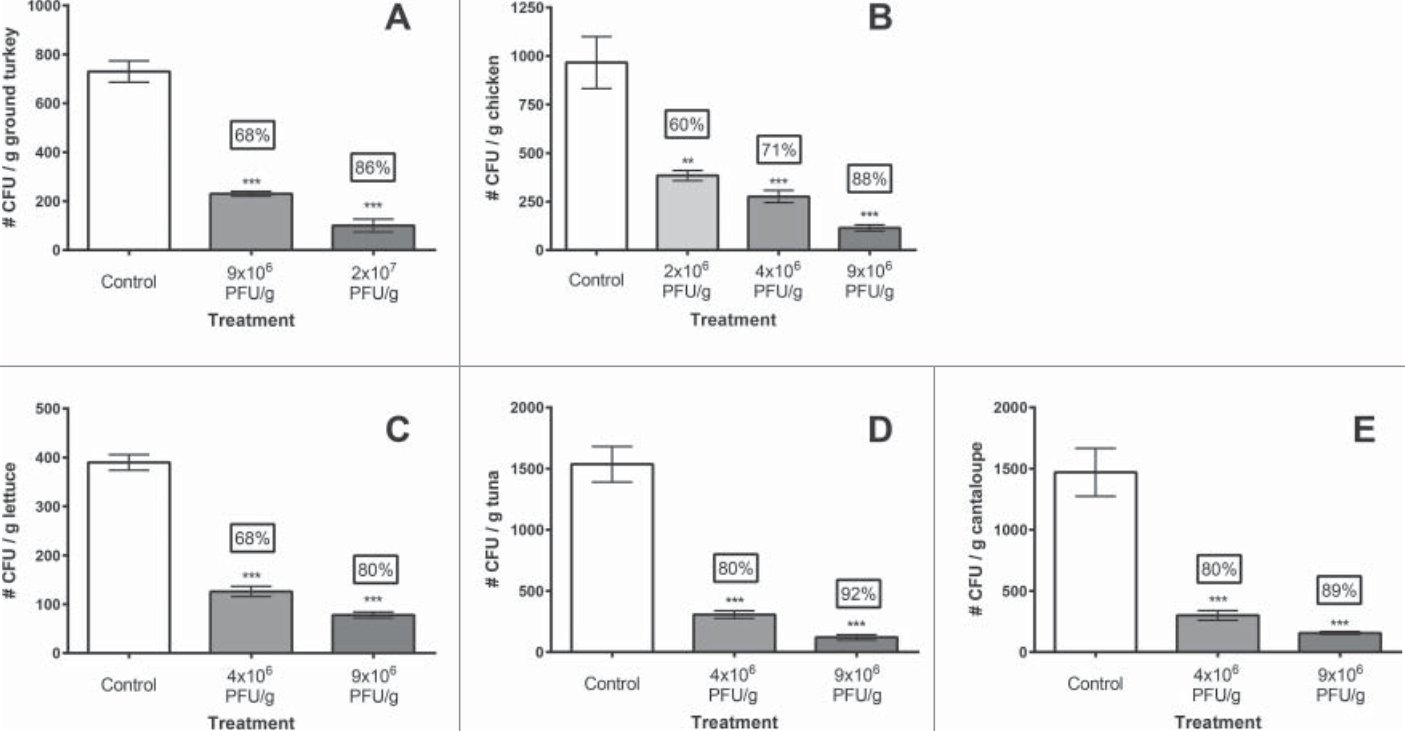
\includegraphics[width=0.5\linewidth]{Plots/Sourced/SalmoFresh_in_pet_food.png}
    \caption{SalmoLyse\textsuperscript{\textregistered} reduces Salmonella contamination on various food surfaces: Mean and standard error bars shown.
        Statistical analyses were carried out for each food group independently.
        Asterisks denote significant reduction from corresponding controls based on one-way ANOVA with Tukey's post-hoc tests for multiple corrections: ** denotes $p < 0.01$, while *** denotes $p < 0.001$ compared to the corresponding controls.
        There was significant reduction in Salmonella on all food surfaces with the addition of SalmoLyse\textsuperscript{\textregistered} compared to the controls; the mean percent reductions from the control are noted in the boxes above treatment bars.
        CFU/g D colony forming units per gram.
        Each letter denotes a food group that was tested with SalmoLyse\textsuperscript{\textregistered} and compared to a control: A= chicken; B= lettuce; C= tuna; D= cantaloupe; E= ground turkey \cite{sofferBacteriophagesSafelyReduce2016}. 
    }
    \label{fig:SalmoFresh_pet_food}
\end{figure}

% TODO: Add section about what phages actually do in the environment (like 20% lysed daily), 
\begin{figure}[ht!]
    \centering
    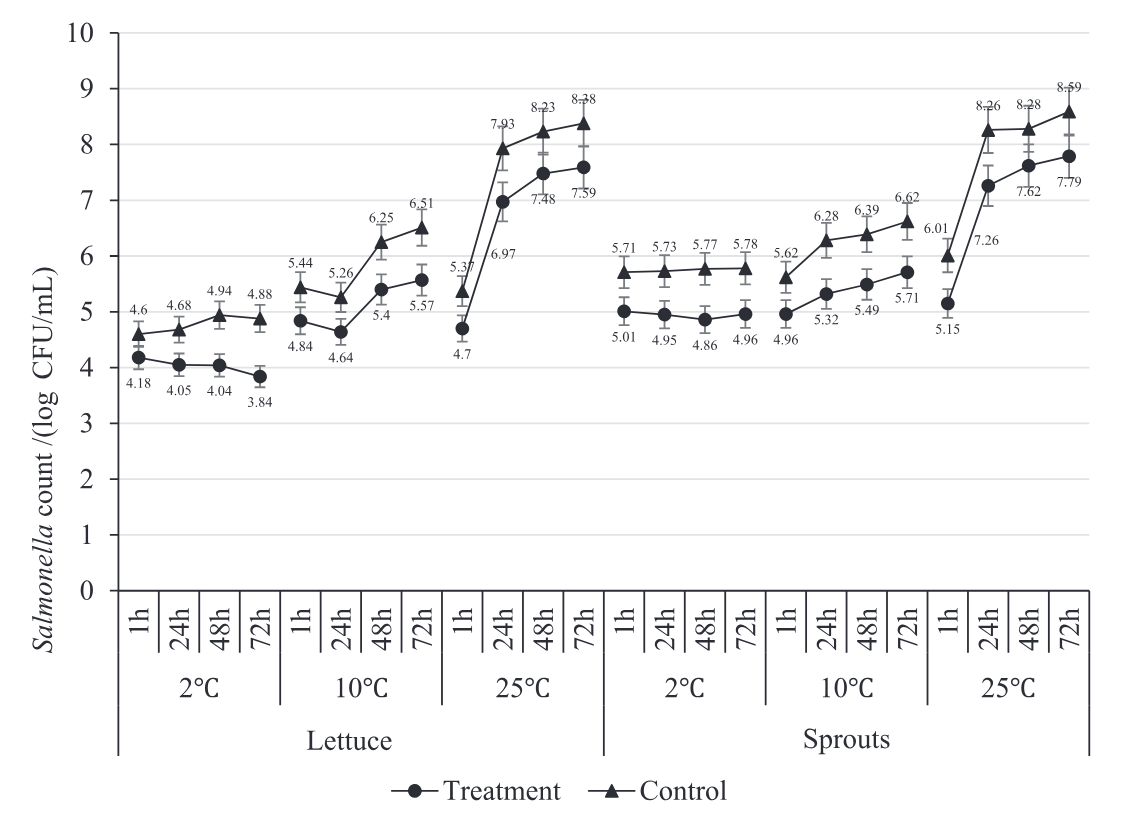
\includegraphics[width=0.5\linewidth]{Plots/Sourced/SalmoFresh_effectiveness_lettuce_sprouts.png}
    \caption{\textit{Salmonella} count in a mixture of 5 \textit{Salmonella} strains spot-inoculated (CFU/g) onto a) lettuce and b) sprouts after spraying with a mixture of bacteriophage (SalmoFresh\textsuperscript{TM}) relative to positive controls at 2, 10 and 25C and stored for 1, 24, 48 and 72 h. \cite{zhangSalmoFreshEffectivenessControlling2019}}
    \label{fig:SalmoFresh_lettuce}
\end{figure}


\section{Phage Therapy and Antibiotics}
\label{sec:AppendixB:phage_therapy_and_antibiotics}
Antibiotics are a common way to treat bacterial infections.
However, antibiotics are not selective in the bacteria they kill, killing both harmful and beneficial bacteria.
This can lead to the development of antibiotic-resistant bacteria, which makes it harder to combat that bacteria in the future.
It has also been shown that antibiotics have a negative effect on the gut microbiome and brain development in mice.
Phages are an alternative to antibiotics, as they are selective in the bacteria they kill and do not interact with cells or other important biological functions.
The rise in antibiotic resistant bacteria can be attributed to the overuse and over-prescription of antibiotics and incorrect usage of antibiotics (for example prematurely stopping) \cite{odonkorBacteriaResistanceAntibiotics2011}.
These actions provide an evolutionary pressure on bacteria to mutate and gain resistance to the antibiotics. 
The phage therapy can contain any number of different phages that can target specific bacterial infections such as \textit{Streptococcus pneumoniae} with minimal risk of side effects.

\subsection{Current Applications: Bacterial Infection Control}
One active area of research is the use of phages to control bacterial infections.
Due to the specificity of phages, they can be used to target specific bacteria strains without affecting other beneficial bacteria.
When sick with a bacterial infection, patients swallow antibiotic pills to help the body fight the infection.
Antibiotics work by either interrupting intercellular processes like the synthesis of RNA \cite{flossRifamycinModeActionResistance2005}, by disrupting the structural integrity of the cell wall \cite{tomaszMechanismIrreversibleAntimicrobial1979}, or by inhibiting protein synthesis \cite{vakulenkoVersatilityAminoglycosidesProspects2003}.

However, antibiotics are not strain specific and indiscriminately kill gut and other bacteria.
Common side effects of antibiotics, although usually not serious, include diarrhea, nausea, and headaches.
It has also been shown that the effects of early-stage penicillin exposure in mice has found to have a long-lasting effect on the gut microbiome, frontal cortex gene expression, and amygdala gene expression \cite{volkovaEffectsEarlylifePenicillin2021}.
Penicillin increases cytokine expression (small proteins used in cell signaling) in the frontal cortex of the brain, modifies the blood-brain barrier integrity, and alters behavior.
The mice exhibited an increase in aggression and anxiety-like behavior \cite{leclercqLowdosePenicillinEarly2017}.
Phages can be used as an alternative to antibiotics without the side effects and without affecting the gut biome. 

With an increase in antibiotic usage, there has been an increase in antibiotic-resistant bacteria.
The World Health Organization has stated that antibiotic resistance threatens the modern medicine and the sustainability of an effective, global public health response to the enduring threat from infectious diseases.
Common infections, that previously would have been easy to treat, are harder to treat, and can increase the risk of disease spread, severe illness, and death \cite{GlobalActionPlan}. 

One area of research is exploring how bacteria can exchange traits such as phage resistance and antibiotic resistance.
Some bacteria are multi-drug resistant, and don't react with the medicine anymore.

\citet{laurePhageResistancemediatedTradeoffs2022} showed evidence that \textit{Salmonella Typhimurium} is more susceptible to ampicillin in the presence of phages, and phage-resistance can lead to reduced virulence and decreased antibiotic resistance. 

\citet{zhaoPhagedrivenCoevolutionReveals2024} showed that there exists an antagonist coevolution between the bacteria and phages, where the dynamics changed from an arms race dynamic (ARD) to a fluctuating selection dynamics (FSD).
Due to phage selection and bacterial competition pressure, when the bacteria gained phage resistance, it lost antibiotic resistance.
A genome analysis revealed mutations in the btuB gene of \textit{Salmonella anatum}, with q higher mutation frequency in the ARD stage.
A knockout experiment confirmed that the btuB gene is a receptor for the JNwz02 phage and resulted in reduced bacterial competitiveness.
Further analysis detected multiple single nucleotide polymorphism (SNP) mutations in the phage-resistant strains.
The SNPs potentially affected the membrane components, partially weakening the cell defense against antibiotics.
These findings help advance our understanding of phage-host-antibiotics interactions and the impact of adaptations to antibiotic resistance.
The research shows how phages can be used to re-introduce antibiotic susceptibility to previous insusceptible bacteria, preventing costly and lengthy research in new antibiotics \cite{zhaoPhagedrivenCoevolutionReveals2024}. 

Phage research is facing challenges due to bacterial strains evolving resistance to phages.
Understanding the interplay between antibiotics and phages is essential for shaping future research \cite{zhaoPhagedrivenCoevolutionReveals2024}.


\section{Environmental Protection}
\label{sec:AppendixB:environmental_protection}
Algae blooms, also called red tides, is the rapid spread of bacterial or algae organisms.
Blooms are a growing environmental concern impacting water quality, aquatic ecosystems, and human health.
These rapid increases in algae populations, often fueled by excess resources like nitrogen and phosphorus, can occur in freshwater, coastal, and marine environment. 

Cyanobacteria blooms have major effects on the aquatic environment as well as human health.
Cyanobacteria release nitrogen and phosphorous, which the bacteria use to grow with oxygen, outpacing other aquatic growth, and killing aquatic marine life.
Bacterial toxins can make their way into the food and water consumed by humans, causing muscle fatigue, respiratory issues, liver damage, and gastrointestinal issues \cite{zhangImpactCyanobacteriaBlooms2022}.
\Cref{fig:cyanobacteria_bloom_cycle} shows the process of how cyanobacteria degrade and are absorbed into the environment, eventually making their way into the human body via various contact points.
 
\begin{figure}
    \centering
    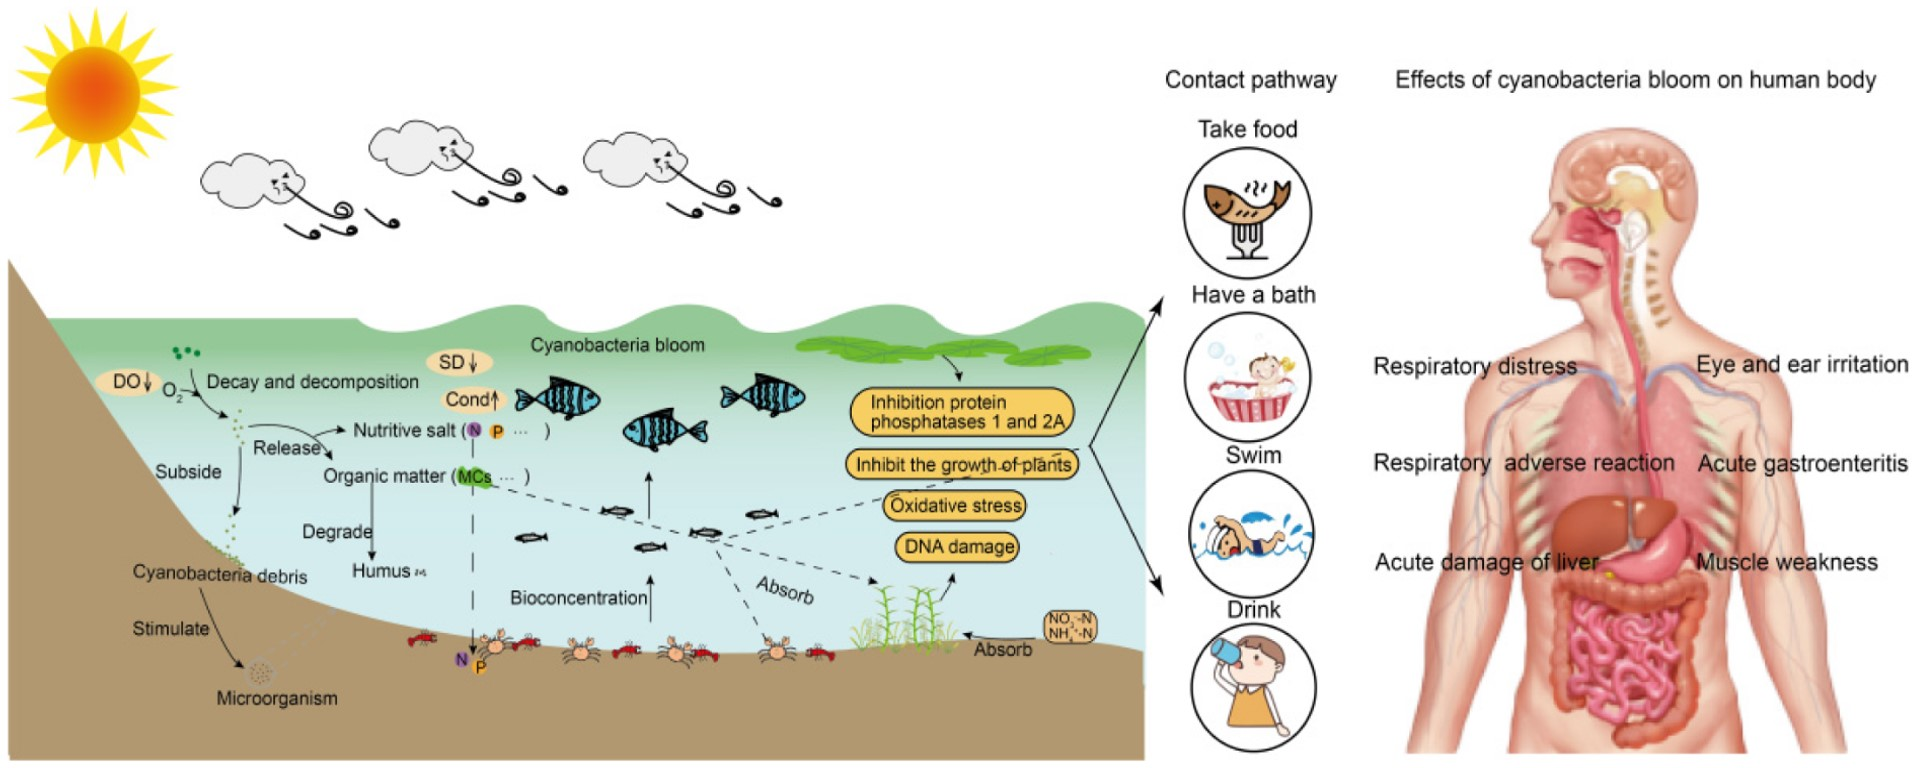
\includegraphics[width=0.75\linewidth]{Figures/cyanobacteria_bloom_cycle.png} 
    \caption{Cyanobacteria degradation cycle, main hazards of cyanobacteria bloom to water bodies, aquatic organisms, and the human body. (DO: dissolved oxygen; SD: water transparency; Cond: conductivity; N: nitrogen; P: phosphorus; MCs: microcystins). \cite{zhangImpactCyanobacteriaBlooms2022}}
    \label{fig:cyanobacteria_bloom_cycle}
\end{figure}

\subsection{Current Applications}
    There is interest in using phages to control cyanobacteria blooms.
Phages can offer better and safer options than chemical options when trying to control bacterial blooms.
Chemical options are indiscriminate, killing cyanobacteria, while also killing other beneficial bacteria and aquatic life, and can eventually seep into groundwater.
Although not used to control bacteria blooms, some chemicals like PFAS, also called “Forever Chemicals”, can last a long time in the environment and don't degrade and keep on negatively affecting the environment.
Due to the specificity of phages, only the cyanobacteria will be targeted, and will not affect the surrounding environment. 

Tucker and Pollard found that an isolated phage cocktail collected from Lake Baroon in Australia could decrease the abundance of \textit{M. aeruginosa} by 95\% within 6 days in a lab setting, before recovering within 3 weeks time \cite{tuckerIdentificationCyanophageMaLBP2005}. \newline
There is evidence that phage-resistant bacteria can influence the population dynamics of other bacteria.
It has been shown that the plankton level has been experimentally affected by the frequency of the phage-resistant \textit{Nodularia} marine bacteria.
Populations with high phage resistance ($>50\%$) dominate the plankton communities despite a high phage count and eventually out compete other bacteria due to their slower loss in population count.
Contrastingly, populations of bacteria with low phage resistance (between 0\% and 5\%) were lysed to extinction, releasing resources like nitrogen.
This allows for other bacterial strains to absorb the resources and dominate the bacterial community.
Phages and the lysis of bacterial strains can have a dramatic effect on community dynamics and composition of other agents like phages, bacteria, and resources \cite{colomaFrequencyVirusresistantHosts2019}.
Phages have the potential to be used as a highly specific strategy for the control of cyanobacterial blooms, with minimal effects to the environment, and offer control of bacterial blooms, with limited impact to the environment.
Usage should be relatively safe, novel, efficient, and sensitive.  

However, there are issues with using phages to control bacterial blooms.
Bacterial blooms can cover vast areas, or be in areas that would be hard to reach like marshlands, applying phages to combat the bloom might be infeasible.
If the method of choice was to spray a solution of water containing phages, the solution needs to be shipped to the site and loaded onto special boats to spray the solution into the water, or the trucks need to drive along the shore and spray the solution into the water.

The phage density in the solution will have to be relatively high to quickly combat the bloom.
These problems provide major logistical problems with creating the phages in a lab or factory, transporting the phages, and finally the administration of the phages to the waterways.
Phages can only diffuse through the water, and can't actively swim, so they are dependent on the rate of diffusion and water currents.
This will be difficult in marshlands, where the bacteria can “hide” in the grass and crevices created by aquatic life.
If the bloom is in a high current area, like in a river or a bay, the water can wash the phages away.

Scientists have not yet fully understood the phage infection mechanism, and research into the artificial engineering of phages is limited, making it challenging to conduct studies in this area \cite{grassoReviewCyanophageHost2022, mckindlesDissolvedMicrocystinRelease2020}.\newline 
Algae can produce toxins that threaten wildlife, contaminate drinking water, and disrupt local economies dependent on fishing and tourism.
In the state of Florida, between the years 1995 and 2000, the restaurant and hotel industry lost an estimated $\$6.5$ million to algae blooms.
This accounts for about 25\% of the average total monthly sales revenue in the region from June through October, the months that are most commonly affected by red tide\cite{PDFEconomicImpacts}.
During a red bloom event, hospital diagnoses in the county of Sarasota for pneumonia, gastrointestinal, and respiratory illness increased by 19\%, 40\% and 54\% respectively \cite{chengCharacterizationMarineAerosol2005, kirkpatrickGastrointestinalEmergencyRoom2010}, with a respiratory illness visit costing between $\$0.5$ and $\$4$ million \cite{hoaglandCostsRespiratoryIllnesses2009}. 